\documentclass[tikz,border=10pt]{standalone}
% No extra TikZ libraries needed.
\begin{document}
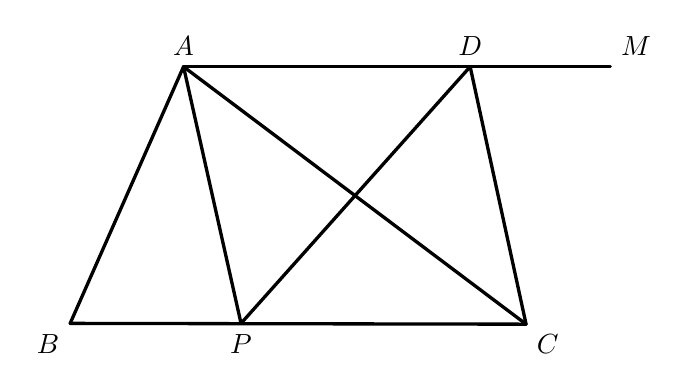
\begin{tikzpicture}[line width=1.2pt, line join=round, line cap=round,
  every label/.style={font=\fontsize{12}{14.4}\selectfont}]
  % Vertices (scale s = 0.015385 cm/px, centred on ink bbox (298,172.5))
  \coordinate (B) at (-3.51,-1.62);
  \coordinate (P) at (-1.34,-1.62);
  \coordinate (C) at (2.28,-1.63);
  \coordinate (A) at (-2.07,1.64);
  \coordinate (D) at (1.57,1.64);
  \coordinate (M) at (3.35,1.64);

  % Bottom line B-P-C
  \draw (B) -- (C);
  % Top line A-D-M
  \draw (A) -- (M);
  % Remaining edges
  \draw (B) -- (A);
  \draw (A) -- (P);
  \draw (A) -- (C);
  \draw (D) -- (P);
  \draw (D) -- (C);

  % Labels
  \node[above] at (A) {$A$};
  \node[above] at (D) {$D$};
  \node[above right] at (M) {$M$};
  \node[below left] at (B) {$B$};
  \node[below] at (P) {$P$};
  \node[below right] at (C) {$C$};
\end{tikzpicture}
\end{document}